\begin{center}
 \begin{minipage}[b]{0.45\textwidth} 
\subsection*{General information}
Name: David Rasmussen \\
Address: Islands brygge 56b 1tv \\
Zip nr. 2300 Koebenhavn S \\
Phone number: 26325635 \\
E-mail: david2300@hotmail.com \\
Country: Danmark \\
Date of birth: 11/06/1995
\newline
 \end{minipage}
 \hfill
\begin{minipage}[b]{4.5cm}
 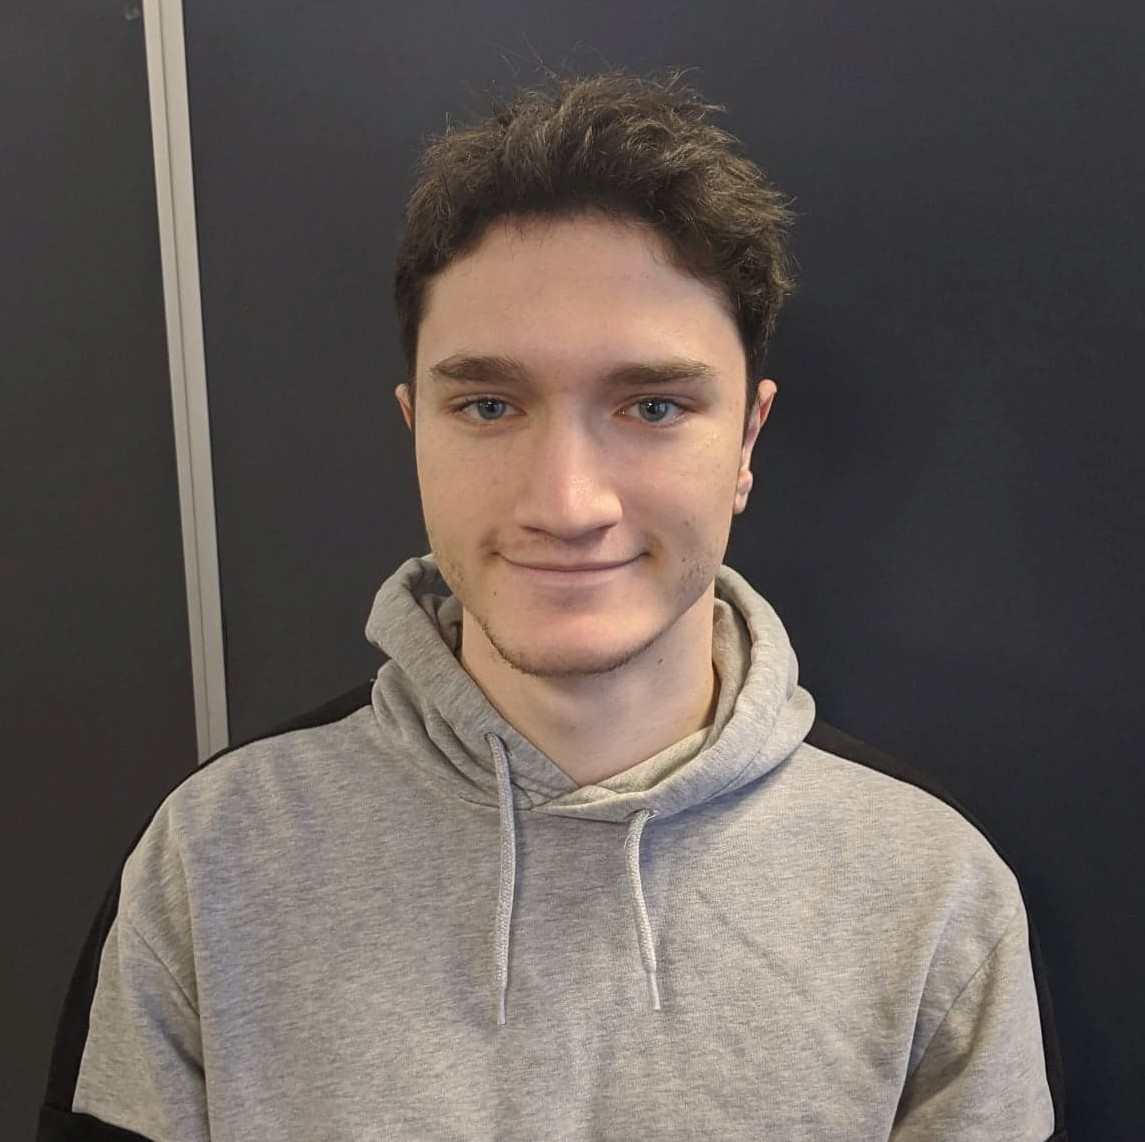
\includegraphics[height=4.25cm]{figures/Billede_af_David}
 \end{minipage}
 \end{center}

\section*{Work experience}
\begin{itemize}
\item 2010 - 2012 Netto - Sevice employee
\item 2012 - 2013 Bauhaus Valby - Salesman
\item 2013 - 2014 Q8 - Sales Assistant
\item 2016 - 2018 Elgiganten Glostrup - Cross operation 
\item 2018 - 2020 Concept - Client service 
\end{itemize}
\section*{Education}
\begin{itemize}
\item 2011 - 2014 HTX-Hilleroed, Biotech
\item 2015 - 2018 Aalborg university Bachelor of Software Engineering
\item 2018 - 2020 Aalborg university Master of Software Engineering
\end{itemize}

\section*{Background Information}
Fluent in english and danish.\\Highschool exam project was using c sharp (unity) to make a game.\\Elementary understand of business and economics.\\Taken courses in analysis.\\Lots of skills in programming.\\Good fundamental understanding of databases.\\Large interest in electronics. Done multiple projects.\\Through university, i have learned c in depth.\\Proficient in C++.\\Once made an embedded electronic watch/thermometer for my girlfriend.\\Taken a BSc and MSc degree in software engineering.\\Did a multi group project, which made me good at agile and large scale software development.\\Experience using Git as a resource management tool.\\Done a lot of lowlevel programming, including: microproccessor programming, and using the language C.\\
